% This is LLNCS.DEM the demonstration file of
% the LaTeX macro package from Springer-Verlag
% for Lecture Notes in Computer Science,
% version 2.4 for LaTeX2e as of 16. April 2010
%
\documentclass{llncs}
\usepackage{algorithm}
\usepackage{algorithmic}
\usepackage{epsfig}
\usepackage{graphicx}
\usepackage{xcolor}
\usepackage{amsfonts,amsmath,amssymb}
\usepackage{fixltx2e} % Fixing numbering problem when using figure/table* 
\usepackage{booktabs}

%
\usepackage{makeidx}  % allows for indexgeneration
%
\begin{document}
%
\mainmatter              % start of the contributions
%
\title{Timeseries features discovery with SAX, TF-IDF weighting and Vector Space model.}
%
\titlerunning{Timeseries features discovery with SAX and TF-IDF weighting}  % abbreviated title (for running head)
%                                     also used for the TOC unless
%                                     \toctitle is used
%
\author{Pavel Senin\inst{1}
\and Sergey Malinchik\inst{2}
}
%
\authorrunning{Pavel Senin} % abbreviated author list (for running head)
%
%%%% list of authors for the TOC (use if author list has to be modified)
%\tocauthor{Ivar Ekeland, Roger Temam, Jeffrey Dean, David Grove,
%Craig Chambers, Kim B. Bruce, and Elisa Bertino}
%
\institute{Collaborative Software Development Laboratory,\\
Information and Computer Sciences Department,\\
University of Hawaii at Manoa,\\ Honolulu HI 96822, USA,\\
\email{senin@hawaii.edu}
\and
Lockheed Martin Corporation,\\
3 Executive campus, Cherry Hill, NJ 08002, USA,\\
\email{sergey.b.malinchik@lmco.com}}


\maketitle              % typeset the title of the contribution

\begin{abstract}
Ability to discover characteristic features in time series paves the road 
for many downstream analyses such as classification and clustering while 
enabling interpretability of results.

In this paper we propose a novel method for time series features discovery 
based on two existing techniques - Symbolic Aggregate Approximation (SAX) 
and Vector space model. This method is capable of discovering and ranking of 
time series features by their ``importance'' to the class - which provides 
interpretable class generalization and facilitates clustering.

The accuracy of this technique, as shown through experimental evaluation, 
is matching or superior to the current state of the art. While being 
computationally expensive within a training phase, our method provides fast 
and interpretable classification.

\keywords{Knowledge discovery, Algorithms, Experimentation}
\end{abstract}
%
\section{Introduction}
%
Time series classification is an increasingly popular area of the research.
While there are numerous algorithms proposed within recent years, to date,
the most robust method is the simple nearest neighbor algorithm (KNN), 
which is simple, and depends on a very few parameters \cite{ed}. 
However, while being virtually unbeatable in performance, kNN algorithm 
requires vast amounts of space and computational time. 
Another drawback is that it provides a very little information about why 
the particular time-series was assigned to a particular class except to 
their mutual distance metrics.

As an alternative to kNN algorithm, recently, time series shapelets were
introduced \cite{shapelet}. A shapelet is a time series subsequence that 
is representative of class membership.
Instead of iteratively looking for the closest neighbor
among all known instances, shapelets-based approaches classifies unknown 
sequences by use of a multivarate decision-tree that supports branching
based on conjunctions or disjunctions of shapelets \cite{logical}. 
While demonstrating a superior interpretability, and similar to kNN algorithms 
performance, shapelets-based approaches are outperformed by other classifiers
and require some additional tuning. Moreover, the approach is relatively
time-consuming.

In this work, we propose a somewhat similar to shapelets technique,
which finds time series subsequences that are representatives of classes.
However, instead of recursive search, our technique is based on the 
single-pass features extraction and their further statistical discrimination,
yielding vectors of all weighted class representatives at once.

\section{Background}
Our methodology is based on two well-known techniques. The first technique is Symbolic
Aggregate approXimation \cite{sax}, which is a high-level, low-bounding symbolic 
representation of time series data. The second technique is a Vector Space model and
\textit{tf$\ast$idf} statistics (weighting), well known in IR field \cite{tfidf}.

\subsection{Symbolic Aggregate approXimation (SAX)} \label{sax}

\begin{figure}[tb]
   \centering
   \includegraphics[height=35mm]{figures/sax_intro.eps}
   \caption{The illustration of the SAX approach taken from \cite{sax} depicts 
    two pre-determined breakpoints for the three-symbols alphabet and the conversion of the time-series of 
    length $n=128$ into PAA representation followed by mapping of the PAA coefficients into SAX symbols with 
    $w=8$ and $a=3$ resulting in the string \textbf{baabccbc}.}
   \label{fig:sax_intro}
\end{figure}

\subsection{TF-IDF weighting scheme} \label{tfidf}
The weighting scheme, that we have used, is a reference \textit{tf$\ast$idf} weighting statistics,
which is defined for a term $t$ and document $D$ 
as a product of a logarithm of a raw term frequency in a document $D$:
\begin{equation}
 \mbox{w}_{t, D} =  \begin{cases} 1 + \log(\mbox{tf}_{t,D}), & \mbox{if } tf_{t,D}>0  \\ 0, & \mbox{otherwise } \end{cases}
\end{equation} 
and a logarithm of an inverse document frequency for that term:
\begin{equation}
 idf_{t} =  \log_{10}(\frac{N}{\mbox{df}_{t}})
\end{equation} 


\subsection{Classification} \label{sax}
\begin{algorithm}
\caption{Class Bag of Words construction}
\label{alg1}
\begin{algorithmic}[1]
\REQUIRE A dataset $D$ containing at least one time series
\ENSURE Return a class WordBag
\STATE $W \leftarrow$ sliding window size
\STATE $P \leftarrow$ PAA size
\STATE $A \leftarrow$ SAX alphabet size
\STATE $B \leftarrow$ \{the resulting bag\}
\FOR{ $t$ in $D$}
 \FOR{ $i\leftarrow 1$ to $|t|-W$}
 \STATE $w \leftarrow SAX(subseries(t,i,W), P, A))$ \{convert subseries into word\}
 \STATE $B \leftarrow w$ \{put the word into the bag, updating frequency\}
 \ENDFOR
\ENDFOR
\RETURN $B$
\end{algorithmic}
\end{algorithm}


\section{Conclusion}
In our opinion, the superior classification performance of our approach is based on 
a number of factors. 
First of all, our approach is very different in nature from those 
based on convenient distance measures such as Euclidean distance or DTW - to some 
extent we do not pay attention to ordering of time points outside of sliding window. 
Surely, overlapping windows do carry information about initial ordering, but this 
is fading away along the steps of our algorithm.
Secondly, we are able to efficiently tolerate noise by leveraging agglomeration 
and mediation with PAA. 
Thirdly, the SAX alphabet cuts provide flexible boundaries for capturing similar 
sub-series. 
And finally, Vector space model and textit{tf$\ast$idf} statistics provide us 
with efficient discrimination and measurement toolkit: the tf part of the weighting scheme
captures the frequency of observed feqtures within the class, while the idf part 
captures the feature informativeness (features that appear in many classes 
are less informative than those that appear rarely)

%
% ---- Bibliography ----
%
\begin{thebibliography}{5}
%

\bibitem {ed}
Ding, H., Trajcevski, G., Scheuermann, P., Wang, X., Keogh, E.:
Querying and mining of time series data: experimental comparison of representations and distance measures,
Proc. VLDB Endow., 1542--1552 (2008)

\bibitem {shapelet}
Ye, L., Keogh, E.:
Time series shapelets: a new primitive for data mining.
Proceedings of the 15th ACM SIGKDD international conference on Knowledge discovery and data mining,
Paris, France, 947--956, (2009)

\bibitem {logical}
Mueen, A., Keogh, E., Young, N.:
Logical-shapelets: an expressive primitive for time series classification.
Proceedings of the 17th ACM SIGKDD international conference on Knowledge discovery and data mining,
San Diego, California, USA, 1154--1162, (2011)

\bibitem {sax}
Lin, J., Keogh, E., Wei, L., Lonardi, S.:
Experiencing SAX: a novel symbolic representation of time series.
Data Mining and Knowledge Discovery, 107--144, (2007)

\bibitem {tfidf}
Salton, G., Wong, A., Yang., C.S.,:
A vector space model for automatic indexing. 
Commun. ACM 18, 11, 613--620, (November 1975)

\end{thebibliography}

%\clearpage
%\addtocmark[2]{Author Index} % additional numbered TOC entry
%\renewcommand{\indexname}{Author Index}
%\printindex
%\clearpage
%\addtocmark[2]{Subject Index} % additional numbered TOC entry
%\markboth{Subject Index}{Subject Index}
%\renewcommand{\indexname}{Subject Index}
%\input{subjidx.ind}
\end{document}
